\scanpage{78}
\mspage{77}
\unsure{\rlap{d}O|O|o}n the other hand, we have an obvious torsor $P_{\unsure{o|0}}$ over $\handwritten{\underline}{Q}_p$ with group $(\handwritten{\hat}{\handwritten{\underline}{Z}})_{\inserted{\handwritten{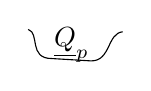
\begin{tikzpicture}[baseline=(q.base),x=1cm,y=1cm]\node[inner sep=0pt] (q) at (0,0) {$\underline{Q}_p$};\draw[thin] (-.55,.2)..controls(-.4,.15)and(-.55,-.17)..(-.25,-.17)--(.25,-.2)..controls(.5,-.2)and(.45,.15)..(.65,.17);\end{tikzpicture}}}}$, corresponding to the maximal unramified extension of $\handwritten{\underline}{Q}_p$ ; \deleted{d}we\deleted{t} take the image \inserted{$P$}\handwritten{\begin{tikzpicture}[baseline=0cm,x=1cm,y=1cm]\draw[thin] (0,-.24)..controls(.08,0)and(.23,.16)..(.29,.53);\end{tikzpicture}} of this torsor: that is it.

8.3. Let $\handwritten{\underline}{H}$ be the kernel gerbe of (8.2.1), which thus has as its band the diagonalizable group $H$ of 8.1. By the general sorites (reference) the class
\margin{\handwritten{$\underline{H}$ is also the \uline{gerbe of liftings}, \uline{for the homomorphism}
\diagram{\begin{tikzcd}[ampersand replacement=\&,column sep=small,row sep=small]
j:\ \underline{G}(F_p) \arrow[r] \arrow[d,phantom,"\simeq"{rotate=90}] \& \underline{\Pi}_p(F_p) \arrow[d,phantom,"\simeq"{rotate=90}] \\
[G] \& [G']
\end{tikzcd}}
deduced from the homomorphism $G\longrightarrow G'$, of the torsor $P$ above.}}
\[
\handwritten{\xi\in}H^{\handwritten{2}}(\handwritten{\underline}{Q}_p,\deleted{\underline{G}_m)}\ H)=\operatorname{Hom}(\handwritten{\underline}{Q},\operatorname{Br}(\handwritten{\underline}{Q}_p))=\operatorname{Hom}(\handwritten{\underline}{Q},\handwritten{\underline}{Q}/\handwritten{\underline}{Z})
\]
of this gerbe is given by
\[
\handwritten{\xi=\partial(\eta)}
\]
where
\[
\handwritten{\eta\in}H^{\handwritten{1}}(\handwritten{\underline}{Q}_p,G')
\]
is the class of the torsor $P$. To car\unsure{\rlap{e}r|r}y out the calculation, note that we have a \deleted{subgroup}\inserted{\unsure{\rlap{e}q|q}\unsure{\rlap{d}u|\rlap{r}u|u}otient} $H'$ of $G_r$, corresponding to the subgroup of $\deleted{\unsure{Q_p|\underline{Q}_p}}$ $\handwritten{\overline}{\handwritten{\underline}{Q}}_p^{\handwritten{*}}$ \deleted{\unsure{formed|formed}} generated by the ro\unsure{\rlap{n}o|o}\unsure{\rlap{e}t|t}s of unity(= torsion elements) and all the roo\unsure{\rlap{n}t|t}s \unsure{\rlap{P}o|\rlap{D}o|o}f $p$, $p^{1/n}$ (this group\deleted{\unsure{e|s}} is indeed invariant under $\operatorname{Gal}(\handwritten{\overline}{\handwritten{\underline}{Q}}_p/\handwritten{\underline}{Q}_p)$ ). We then have a homomorphism of extensions
\margin{\handwritten{\uline{NB} This diagram is induced by a diagram of \uline{gerbes} (valid over any perfect field $k$) with $\underline{H}'=$ gerbe corresponding to the subcategory of $\operatorname{Fcriso}(\mathbb{F}_p)$ form\unsure{ed|ed} of the objects which become isomorphic over a \uline{finite} extension $k'$ of $k=\mathbb{F}_p$ to a sum of objects $E_{r,s}$ ; and $H$ is identified with the \uline{gerbe of liftings} of $P_o$ for the homomorphism $j:\underline{H}'\longrightarrow[\hat{\underline{Z}}]$ associated to $H'\longrightarrow(\hat{\underline{Z}})_{\mathbb{Q}_p}$ ...}}
\diagram{\begin{tikzcd}[ampersand replacement=\&]
0 \handwritten{\arrow[r]} \& H \handwritten{\arrow[r]} \handwritten{\arrow[d]} \& G \handwritten{\arrow[r]} \handwritten{\arrow[d]} \& G' \handwritten{\arrow[r]} \handwritten{\arrow[d]} \& 0 \\
0 \handwritten{\arrow[r]} \& H \handwritten{\arrow[r]} \& H' \handwritten{\arrow[r]} \& \handwritten{\unsure{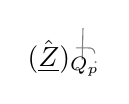
\begin{tikzpicture}[baseline=(z.base),x=1cm,y=1cm]\draw[gray,thin] (.23,-.02)--(.24,.38);\draw[gray,thin] (.15,.13)--(.29,.13)..controls(.36,.14)and(.39,.1)..(.39,.06);\fill[gray] (.4,-.05) circle(.014);\node[inner sep=0pt] (z) at (0,0) {$(\hat{\underline{Z}})_{\mathbb{Q}_p}$};\end{tikzpicture}}} \handwritten{\arrow[r]} \& 0\ ,
\end{tikzcd}}
which shows that \rlap{i}w\rlap{d}e \deleted{suffices to calculate} have
\[
\handwritten{\xi=\partial(\eta_o)},
\]
where
\[
\handwritten{\unsure{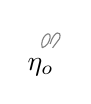
\begin{tikzpicture}[baseline=(e.base),x=1cm,y=1cm]\draw[gray,thin] (.02,.24)..controls(-.02,.37)and(.13,.49)..(.12,.37)..controls(.09,.24)and(.01,.25)..(.02,.24);\draw[gray,thin] (.12,.29)..controls(.17,.46)and(.27,.47)..(.24,.36)--(.15,.24);\node[inner sep=0pt] (e) at (0,0) {$\eta_o$};\end{tikzpicture}}\in}H^{\handwritten{1}}(\handwritten{\underline}{Q}_p,\handwritten{\hat}{\handwritten{\underline}{Z}})
\]
is the im\unsure{\rlap{d}a|a}ge of $\handwritten{\eta}$ under $G'\handwritten{\longrightarrow}\handwritten{\hat}{\handwritten{\underline}{Z}}$. We observe that the composite of (8.2.2) with the preceding homomorphism is the identity of $\handwritten{\hat}{\handwritten{\underline}{Z}}$, hence $\handwritten{\unsure{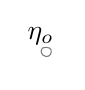
\begin{tikzpicture}[baseline=(e.base),x=1cm,y=1cm]\draw[gray,thin] (.02,-.15)..controls(.2,-.09)and(.14,-.32)..(.03,-.24)..controls(-.01,-.2)and(.01,-.17)..(.02,-.15);\node[inner sep=0pt] (e) at (0,0) {$\eta_o$};\end{tikzpicture}}}$ is the class of the canonical torsor $P_o$ at the end of 8.2. With the help\deleted{d} of this, one must verify that the class $\handwritten{\xi}$ corresponds (under the isomorphism
\[
\operatorname{Br}(\handwritten{\underline}{Q}_p)\handwritten{\simeq}\handwritten{\underline}{Q}_{\deleted{\handwritten{p}}}/\handwritten{\underline}{Z}_{\deleted{\handwritten{p}}}
\]
of \rlap{c}local class field theory, to the canonical homomorphism $\handwritten{\mathbb{Q}\longrightarrow\mathbb{Q}/\mathbb{Z}}$
